\documentclass[12pt,a4paper,oneside]{report}
\usepackage{graphics}
\begin{document}

\title{Extension: Debugger And Extended Instruction Set}
\author{Ganesh Kumar, Jose Kalladanthyil, Varun Verma}
\date{June 2012}
\maketitle

%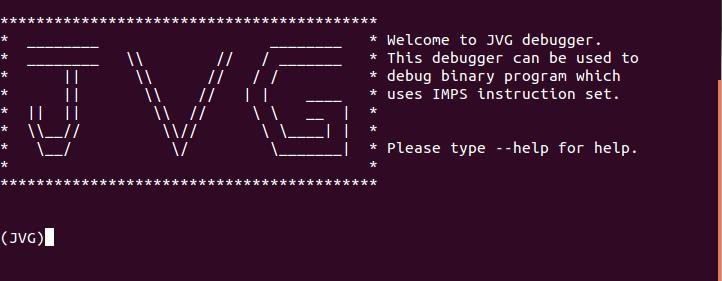
\includegraphics[width=\linewidth]{graphics1.jpg}
%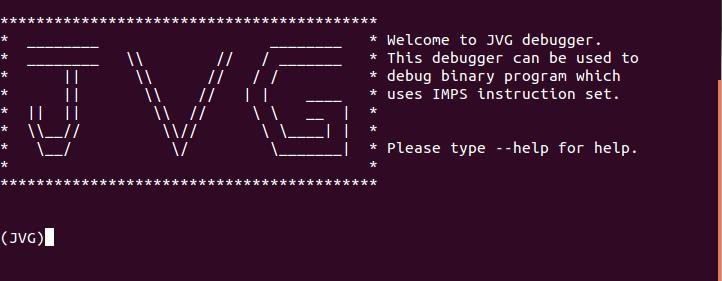
\includegraphics {graphics1.jpg}
\begin{figure}[htb]
\centering
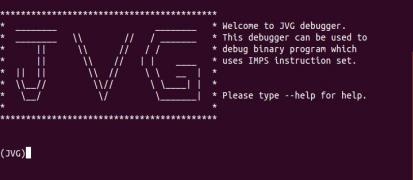
\includegraphics{graphics.jpg}
\caption{Debugger}
\label{fig:awesome_image}
\end{figure}

The debugger JVG has been designed which allows a user to debug their IMPS assembly instrucion programs. The user has various different options which can be chosen at runtime to allow the user to track the error in their program. Once the user enters the debugger, the following welcome message is seen in the terminal.\
The “(JVG)” on the terminal indicates that the debugger is waiting for the user input, i.e. the command from user to carry out a a task. The list of commands can be obtained by typing “--help” which then further guides the user how to use the commands and gives deatiled description of each of the commands which a user is able to use in the JVG debugger.  

The user has following options of commands:
Print and search through some or all registers
Print and search through some or all memory locations
Use breakpoints in the given program
Run a program
Reset the state of processor to the state it was in at the start of program
print contents of the processor in the current state.
Step through the program
quit the debugger
print the current assmbly line which was just executed

The debugger stops the program which is currently running and indicate the user if a segmentation fault could occur by executiong the current command. This is done by checking the instruction is a valid instruction. This involves checking the opcode value to see if it is within range of opcodes which are included in the extended opcode set. The operands values are checked to check they would cause a valid operation or not. This involves checking if carrying out the current operation would result in reading an invalid register or invalid memory location. For eg, if a instruction is trying to load a into register 1 the value stored at memory location 67000 which does not exists, or reading the value of \textdollar 35 which is inexistent since an IMPS processor only has 32 general purpose registers.

The debugger also has extensive checks for each of the input command for debugging  any IMPS program. This excludes the possbilities of invalid commands which could possible cause the debugger to break. The degubber has be made as robust as possible by inlcluding intensive checks before any command is executed or any instrucion is carried out. The possibility of segmentation faults which could be caused due to  broken assembly program is also been eliminated by including checks for the instruction being valid. 

The debugger allows the user to print the current value stored in the program counter of the processor, the current line of code being executed. Other commands allow the user to set breakpoints at certain line numbers in the program currently being run. The list of commands is shown below which can also be obtained by entering the command “--help” in the debugger:\\
\textbullet {\bf list} \\
\textbullet {\bf pc}\\
\textbullet {\bf search}\\
\textbullet {\bf reg}\\
\textbullet {\bf mem}\\
\textbullet {\bf q}\\
\textbullet {\bf break}\\
\textbullet {\bf stp}\\
\textbullet {\bf reset}\\
\textbullet {\bf --help}\\
\textbullet {\bf run}\\
The 'list' command prints the last command which was executed. The 'pc' comamnd prints the current value which is stored in the program counter of the processor. The 'search' command searches for a value in either registers or memory. The flags for the search command specify if the search is carried out in the memory or registers. The user can also search in all registers or all memory location or in the range specified which depends on the flags provided to the search command. The 'reg' command can be used to print value of either specific registers or registers within the speicified range or all registers which can be specified by the flags provided to the command 'reg'. The 'mem' command can be used to print value of either specific memory locations or memory locations within the speicified range or all memory locations which can be specified by the flags provided to the command 'mem'. The 'q' can be used to quit the debugger which asks the user to confirm the quit before exiting the debugger. The 'break' command can be used introduce and remove breakpoints from a  program. The 'stp' command carries out one instruction, this method provides feedback if the program has already been run before in which case 'stp' command cannot be executed. The command 'reset' resets the state of the cpu to the state in which the user can run or stp in the program again. The command '--help' provides the user with the list of commands which can be used in the debugger. The help command then further assists the user in order to allow the user to get the help for certain commands. The 'run' commands the runs the comeplete program.

The extended instruction set now contains the given 19 instructions and also 7 new instructions providing the user with more functionality and easier implementation of some most used functions. The new instructions which have been added are:\\
\textbullet {\bf 'div'} -This is an R-type instruction that makes use of three registers.
div R1 R2 R3 stores in R1 the quotient from the division of R2 by R3\\
\textbullet {\bf 'divi'} -This is an I-type instruction that makes use of two registers and an immediate value. divi R1 R2 I stores in R1 the quotient from the division of R2 and I.\\
\textbullet {\bf 'fact'}- This is an R-type instruction that makes use of two registers.
fact R1 R2 stores in R1 the factorial of the integer stored in R2. \\
\textbullet {\bf 'facti'}- This is an I-type instruction that makes use of one register and an immediate value.
facti R1 R2 I stores in R1 the factorial of the integer I.\\
\textbullet {\bf 'mod'}- This is an R-type instruction that makes use of three registers.
mod R1 R2 R3 stores in R1 the remainder from the division of R2 by R3\\
\textbullet {\bf 'modi'} - This is an I-type instruction that makes use of two registers and an immediate value.
modi R1 R2 I stores in R1 the remainder from the division of R2 and I.\\
\textbullet {\bf 'swap'} - This is an R-type instruction that makes use of two registers. Swap R1 R2 swaps the values held in R1 and R2 so that after the operation R2 is made to hold the previous value of R1 and vice versa.\\



\begin{center}
\section*  {Design}
\end{center}


High-level features like modularity is used in the code. Some of the methods which are common to the debugger and the emulator have been included using the include statements for those header files which provides the implemenation of the complete IMPS project higher modularity. Since if any of the methods whicih has to be changed would only be changed once and not once for each emulator, assembler and debugger. The code for executing all the instruction is in the file 'carryOutInstruction.c', this allows the adding of instructions in the instruction set to be easy. The user can add their own defined functions which might be specific to their tasks. This eliminates the user to still asseemble without changing much of the code for the assembler. 

The main challenge which we encountered as a group when we started doing the function to allow the user to step back. The first solution we though was to make a double linked list and store each state of the processor but this idea was dropped due to the amount of memory which could be used in a program which might have an infinite loop. We could not find any neater solution for this problem. Another challenger was when we wanted to catch if any segmentation fault would occur in the debugger due to the broken assembly code. This would have caused the debugger to crash with a  segmentation fault. After looking into how to design a signal handler in C, as a group we decided to drop the idea of making our own signal handler and carry out checks to check if any segmentation fault could have occurred by checking if all registers and the memory locations being accessed existed. Another functionality of the debugger which we had great great difficulty in implementing was using the up and down arrow keys to get to the previous and the next command. This would have involved to keep a double linked list with a pointer to the current command. We starteded implementing it but then great problems were encountered to read the arrow keys from the terminal.\\



%\begin{center}
\section*{Testing}
%\end{center}


The implementation of the debugger was tested by debugging the test files given. Some of the files were changed to inuclude broken assembly which should exit the program when run with the emulator and cause a segmentation fault. These files were used to test the debugger which allowed to check if all the functionality of the debugger was working. Another technique which we used to test the debugger included making a broken assembly file which was assembled and then the files was given to a team member who was not allowed to see the contents of the assembly instructions in that file and was required to trace the error using the debugger. The error was very trivial. The program was a very simple loop which consisted of a loop which decremented the value of the variat of the loop. Instead of drementing, the variant was incremented rather than decrementing. This caused an infinite loop when the program was emulated. The error was traced using the debugger by carrying out one step at a time by using the command 'stp' and then the state of the register which contained the value for the variant was check and was found to increase. Each of the method which was unique to the debugger was tested by creating a test file for it which ran the method with dummy values to check whether it produces the correct output or not.\\

%\begin{center}
\begin{center}
\section*{Group-Working (Programming in Team)}
\end{center}
%\section* {Group-Working (Programming in Team)}
%\end{center}
Different people in the team had different ideas and different knowledge of the lanuage, this allowed us to learn from each other. Each incdivual of the team was giver certain methods and was required to finish  the methods and test them using dummy parameters and values to check if it method produces the correct output or not. The method were combined together to check for any lnking errors. Good communication between the team was the most important thing since not communicating sometimes caused two people working on the same method or debugging the same methods and changing various things which introduced more errors. Git was very helpful tool since the previous version of the files could be able to retrieved incase any bugs were introduced while debugging. 

\end{document}